\documentclass[../5RO17_TP4.tex]{subfiles}

\begin{document}
\section{Recalage par ICP}
\noindent Comme explique sur la section précedent, la transformation recherchée est celle qui minimise l'erreur quadratique totale donnée par:
\begin{equation}
    f(\mathbf{R}, \mathbf{T}) = \frac{1}{n} \sum_{i=1}^{n} \left[ p_{\text{reference}_i} - (\mathbf{R} \cdot p_{\text{cloud}_i} + \mathbf{T}) \right]^{2}
\end{equation}
Cette fois-ce, nous explorerons la meilleure transformation rigide au sens de la recalage par ICP comme implemente ci-dessous:
\begin{scriptsize}\mycode
	\begin{lstlisting}[language=Python, caption=\texttt{compute\_ICP()}]
def compute_ICP(data, ref, max_iter, RMS_threshold):
    # Variable for aligned data
    data_aligned = np.copy(data)

    # Create a neighbor structure on ref
    search_tree = KDTree(ref.T)

    # Initiate lists
    R_list = []
    T_list = []
    neighbors_list = []
    RMS_list = []

    for i in range(max_iter):
        # Find the nearest neighbors
        distances, indices = search_tree.query(data_aligned.T, return_distance=True)

        # Compute average distance
        RMS = np.sqrt(np.mean(np.power(distances, 2)))

        # Distance criteria
        if RMS < RMS_threshold:
            break

        # Find best transform
        rotation, translation = compute_rigid_transformation(data, ref[:, indices.ravel()])

        # Update lists
        R_list.append(rotation)
        T_list.append(translation)
        neighbors_list.append(indices.ravel())
        RMS_list.append(RMS)

        # Aligned data
        data_aligned = rotation.dot(data) + translation

    return data_aligned, R_list, T_list, neighbors_list, RMS_list
	\end{lstlisting}
\end{scriptsize}

\noindent De cette manière, les résultats suivants ont été obtenus:
\begin{figure}[H]
    \centering
    \begin{subfigure}[b]{0.475\textwidth}
        \centering
        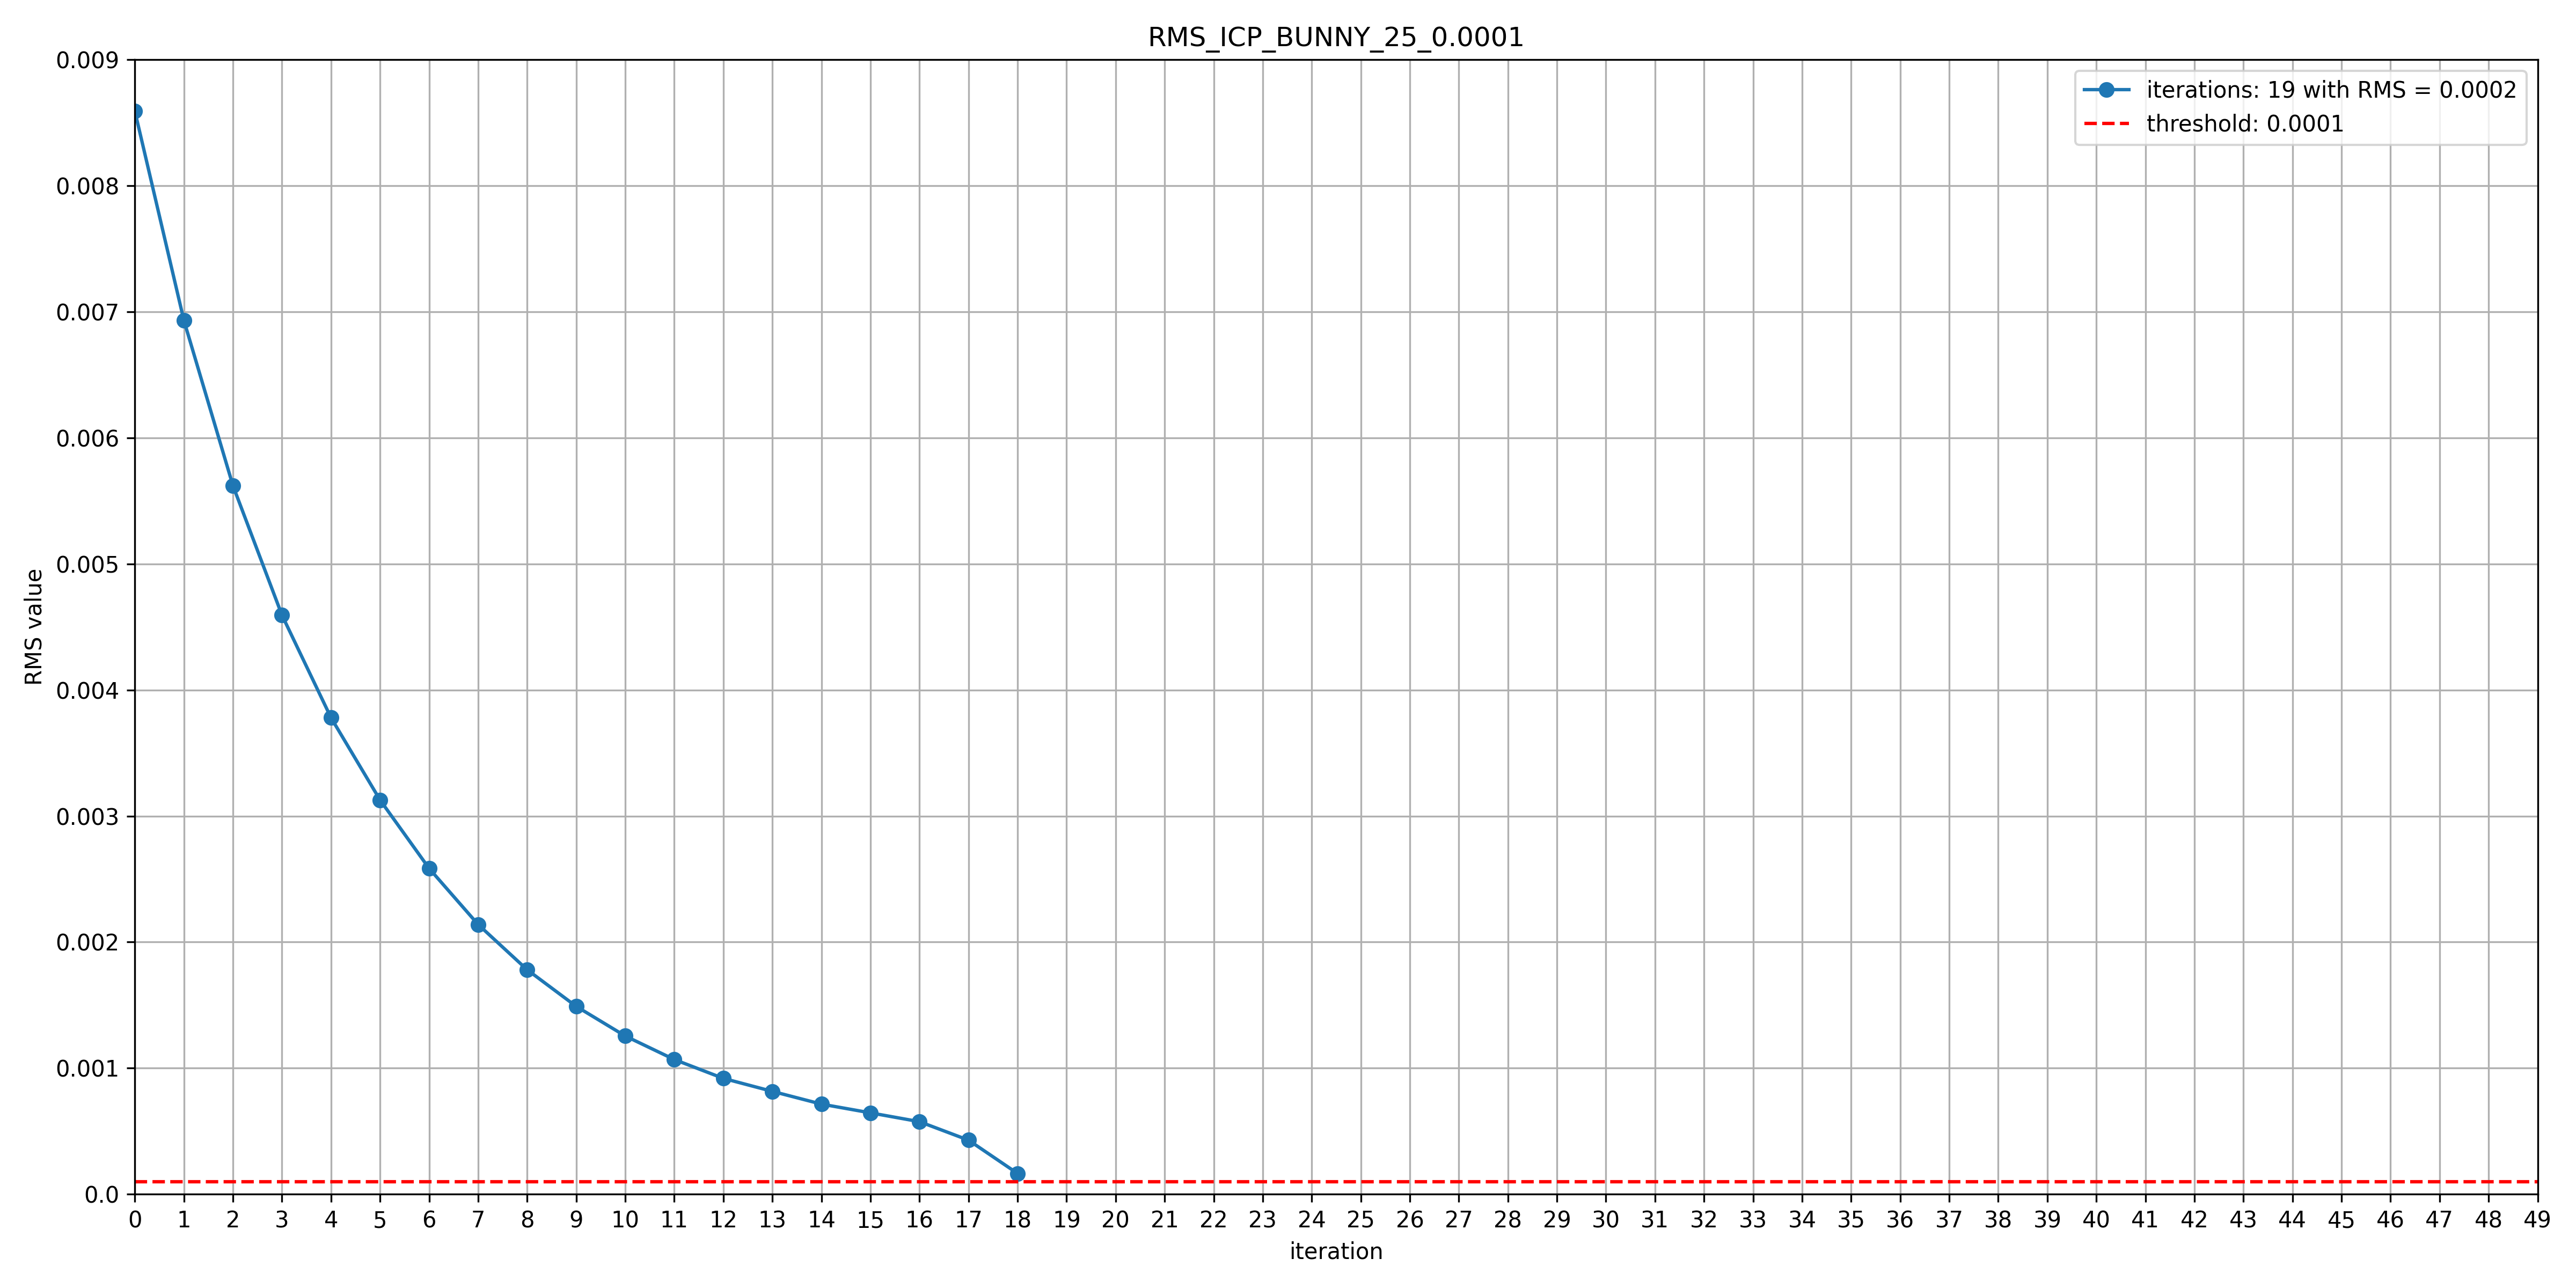
\includegraphics[width=\linewidth]{images/RMS_ICP_BUNNY_25_0.0001.png}
        \caption{\texttt{Bunny} avec 25 iteractions}
        \label{}
    \end{subfigure}\hfill
    \begin{subfigure}[b]{0.475\textwidth}
        \centering
        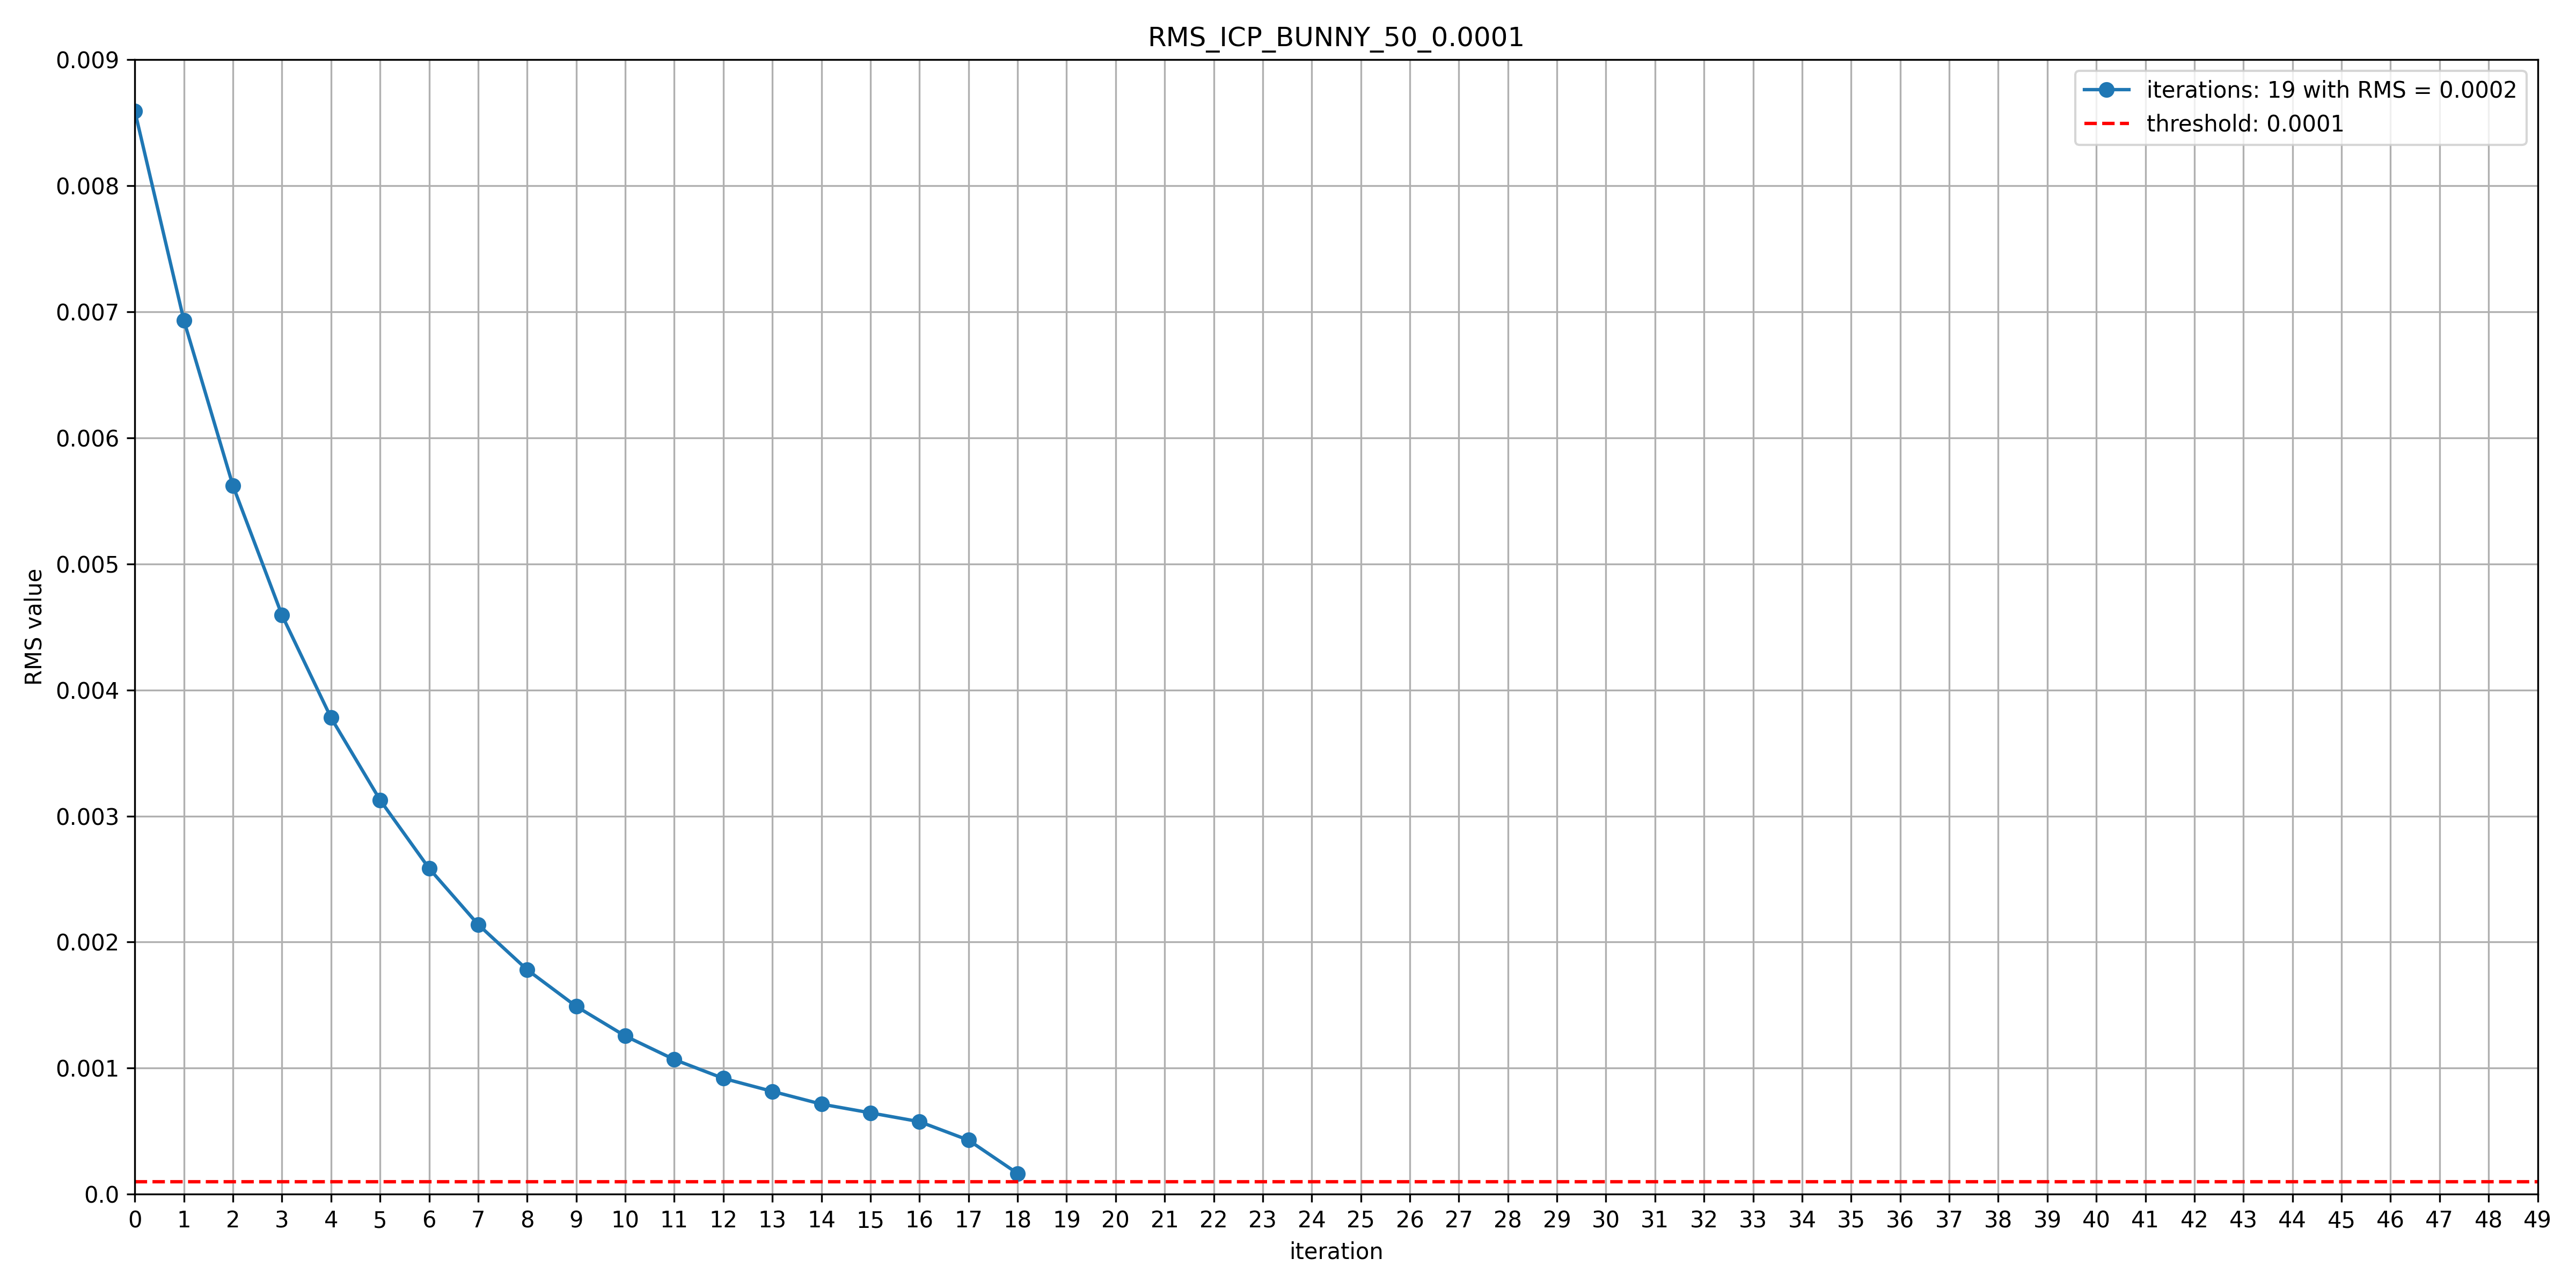
\includegraphics[width=\linewidth]{images/RMS_ICP_BUNNY_50_0.0001.png}
        \caption{\texttt{Bunny} avec 50 iteractions}
        \label{}
    \end{subfigure}\hfill
    \begin{subfigure}[b]{0.475\textwidth}
        \centering
        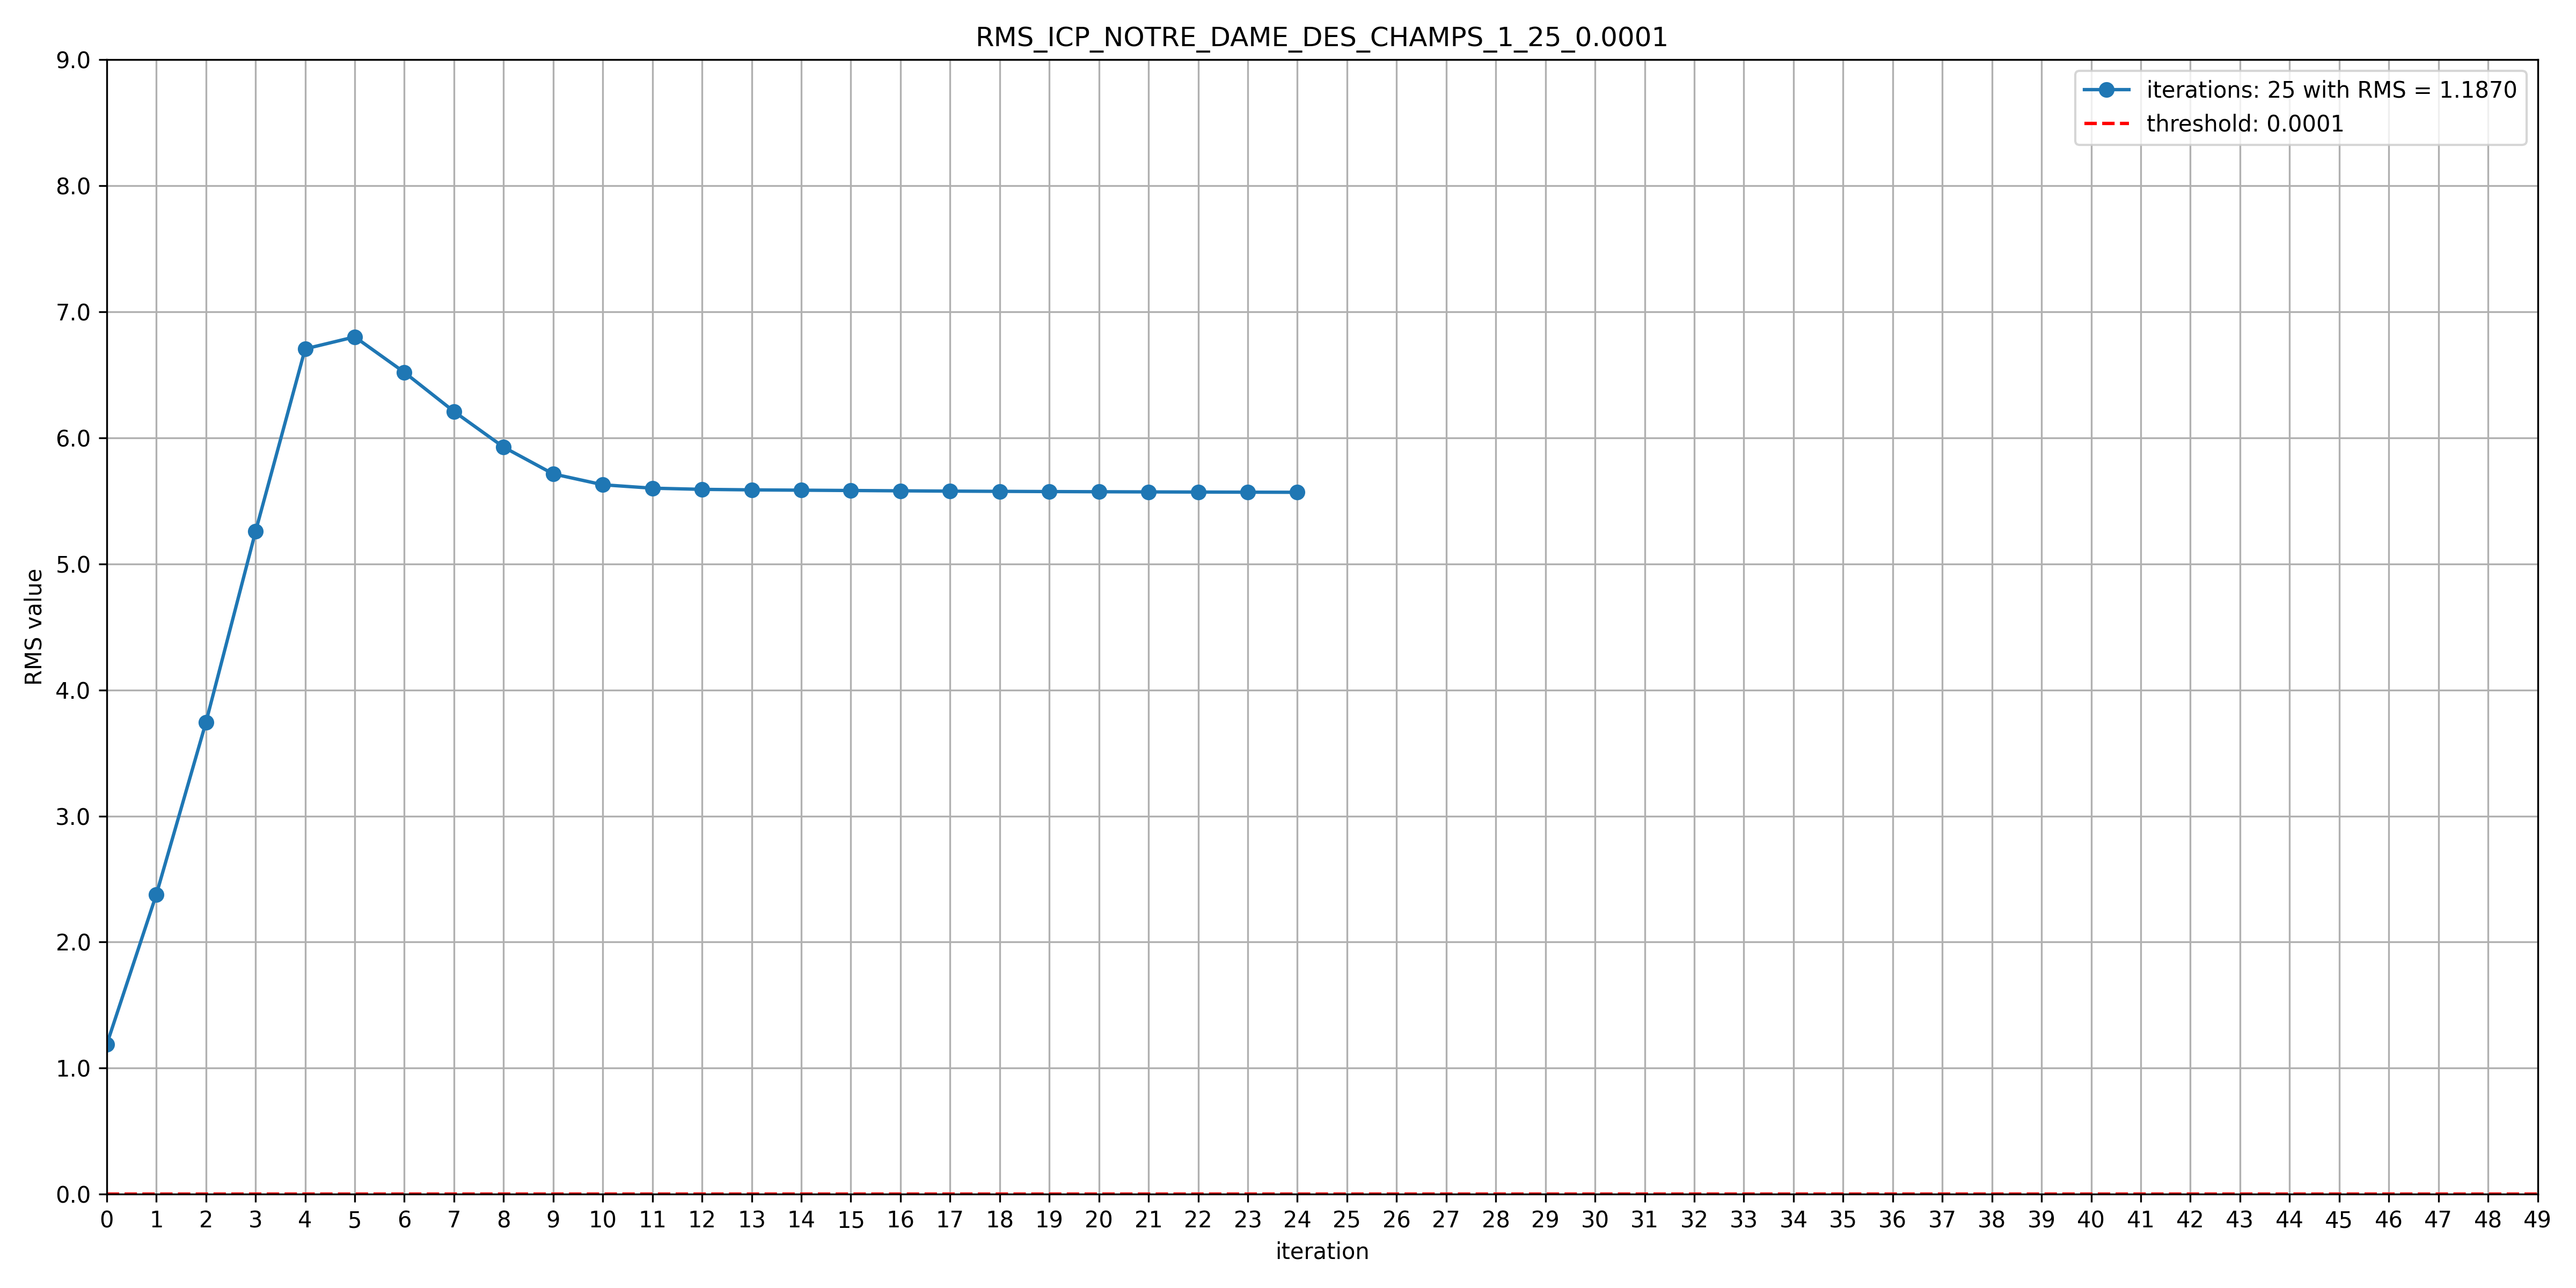
\includegraphics[width=\linewidth]{images/RMS_ICP_NOTRE_DAME_DES_CHAMPS_1_25_0.0001.png}
        \caption{\texttt{NDC} non decimated avec 25 iteractions}
        \label{}
    \end{subfigure}\hfill
    \begin{subfigure}[b]{0.475\textwidth}
        \centering
        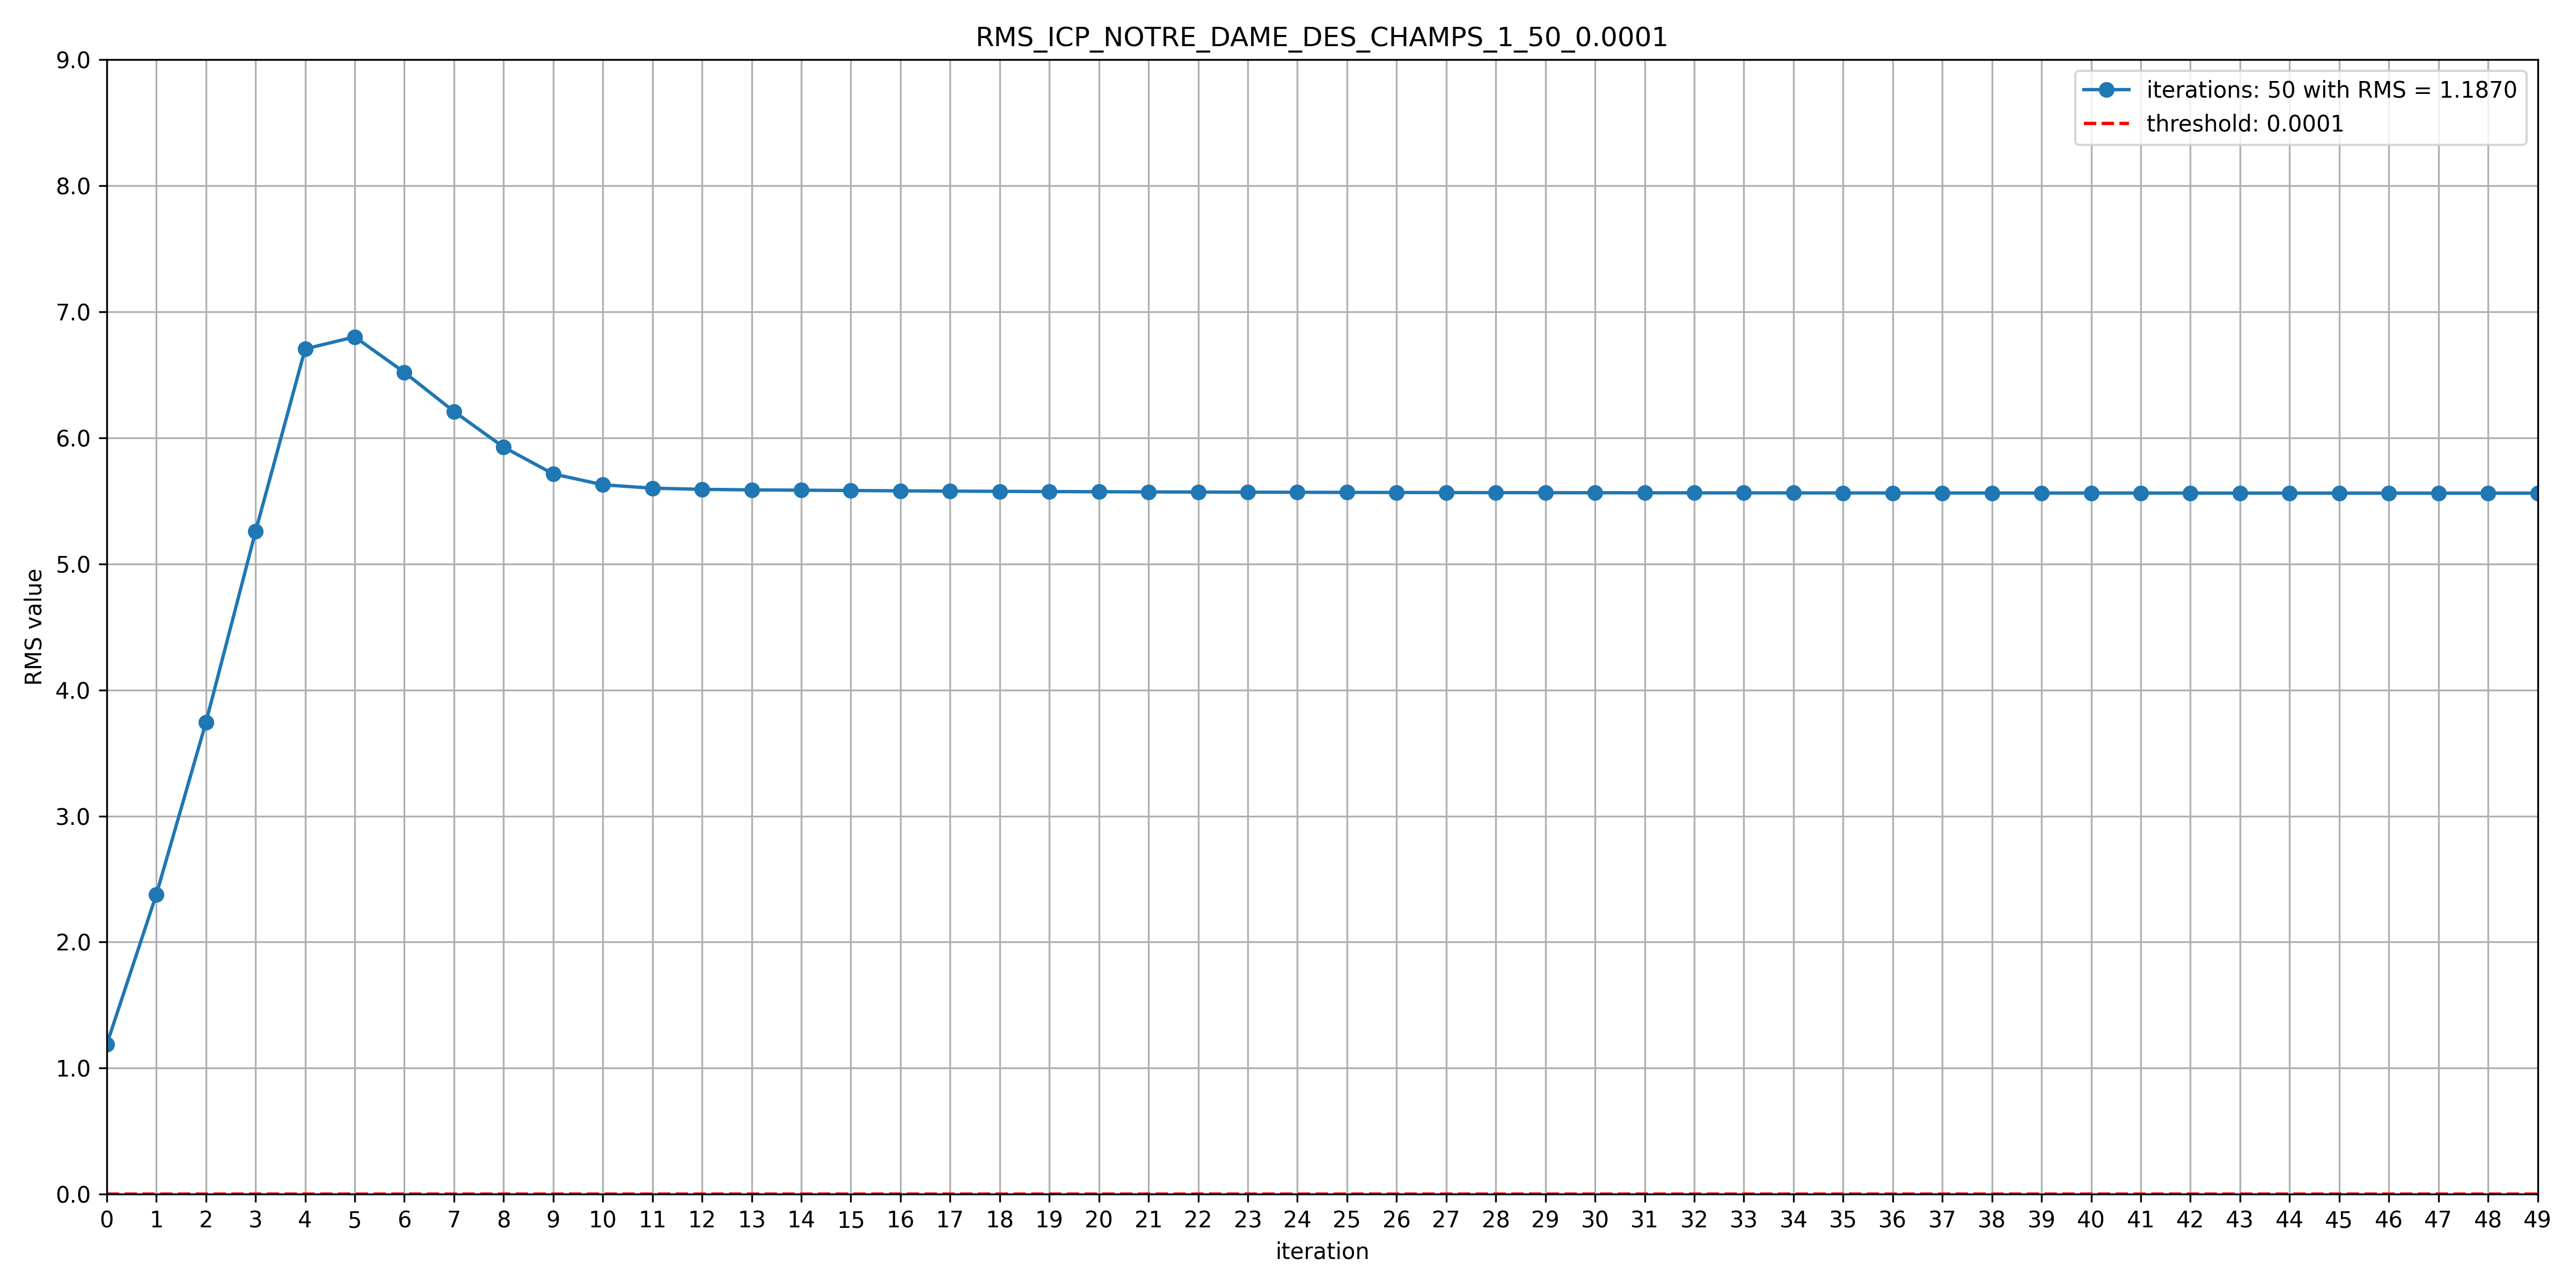
\includegraphics[width=\linewidth]{images/RMS_ICP_NOTRE_DAME_DES_CHAMPS_1_50_0.0001.png}
        \caption{\texttt{NDC} non decimated avec 50 iteractions}
        \label{}
    \end{subfigure}\hfill
    \begin{subfigure}[b]{0.475\textwidth}
        \centering
        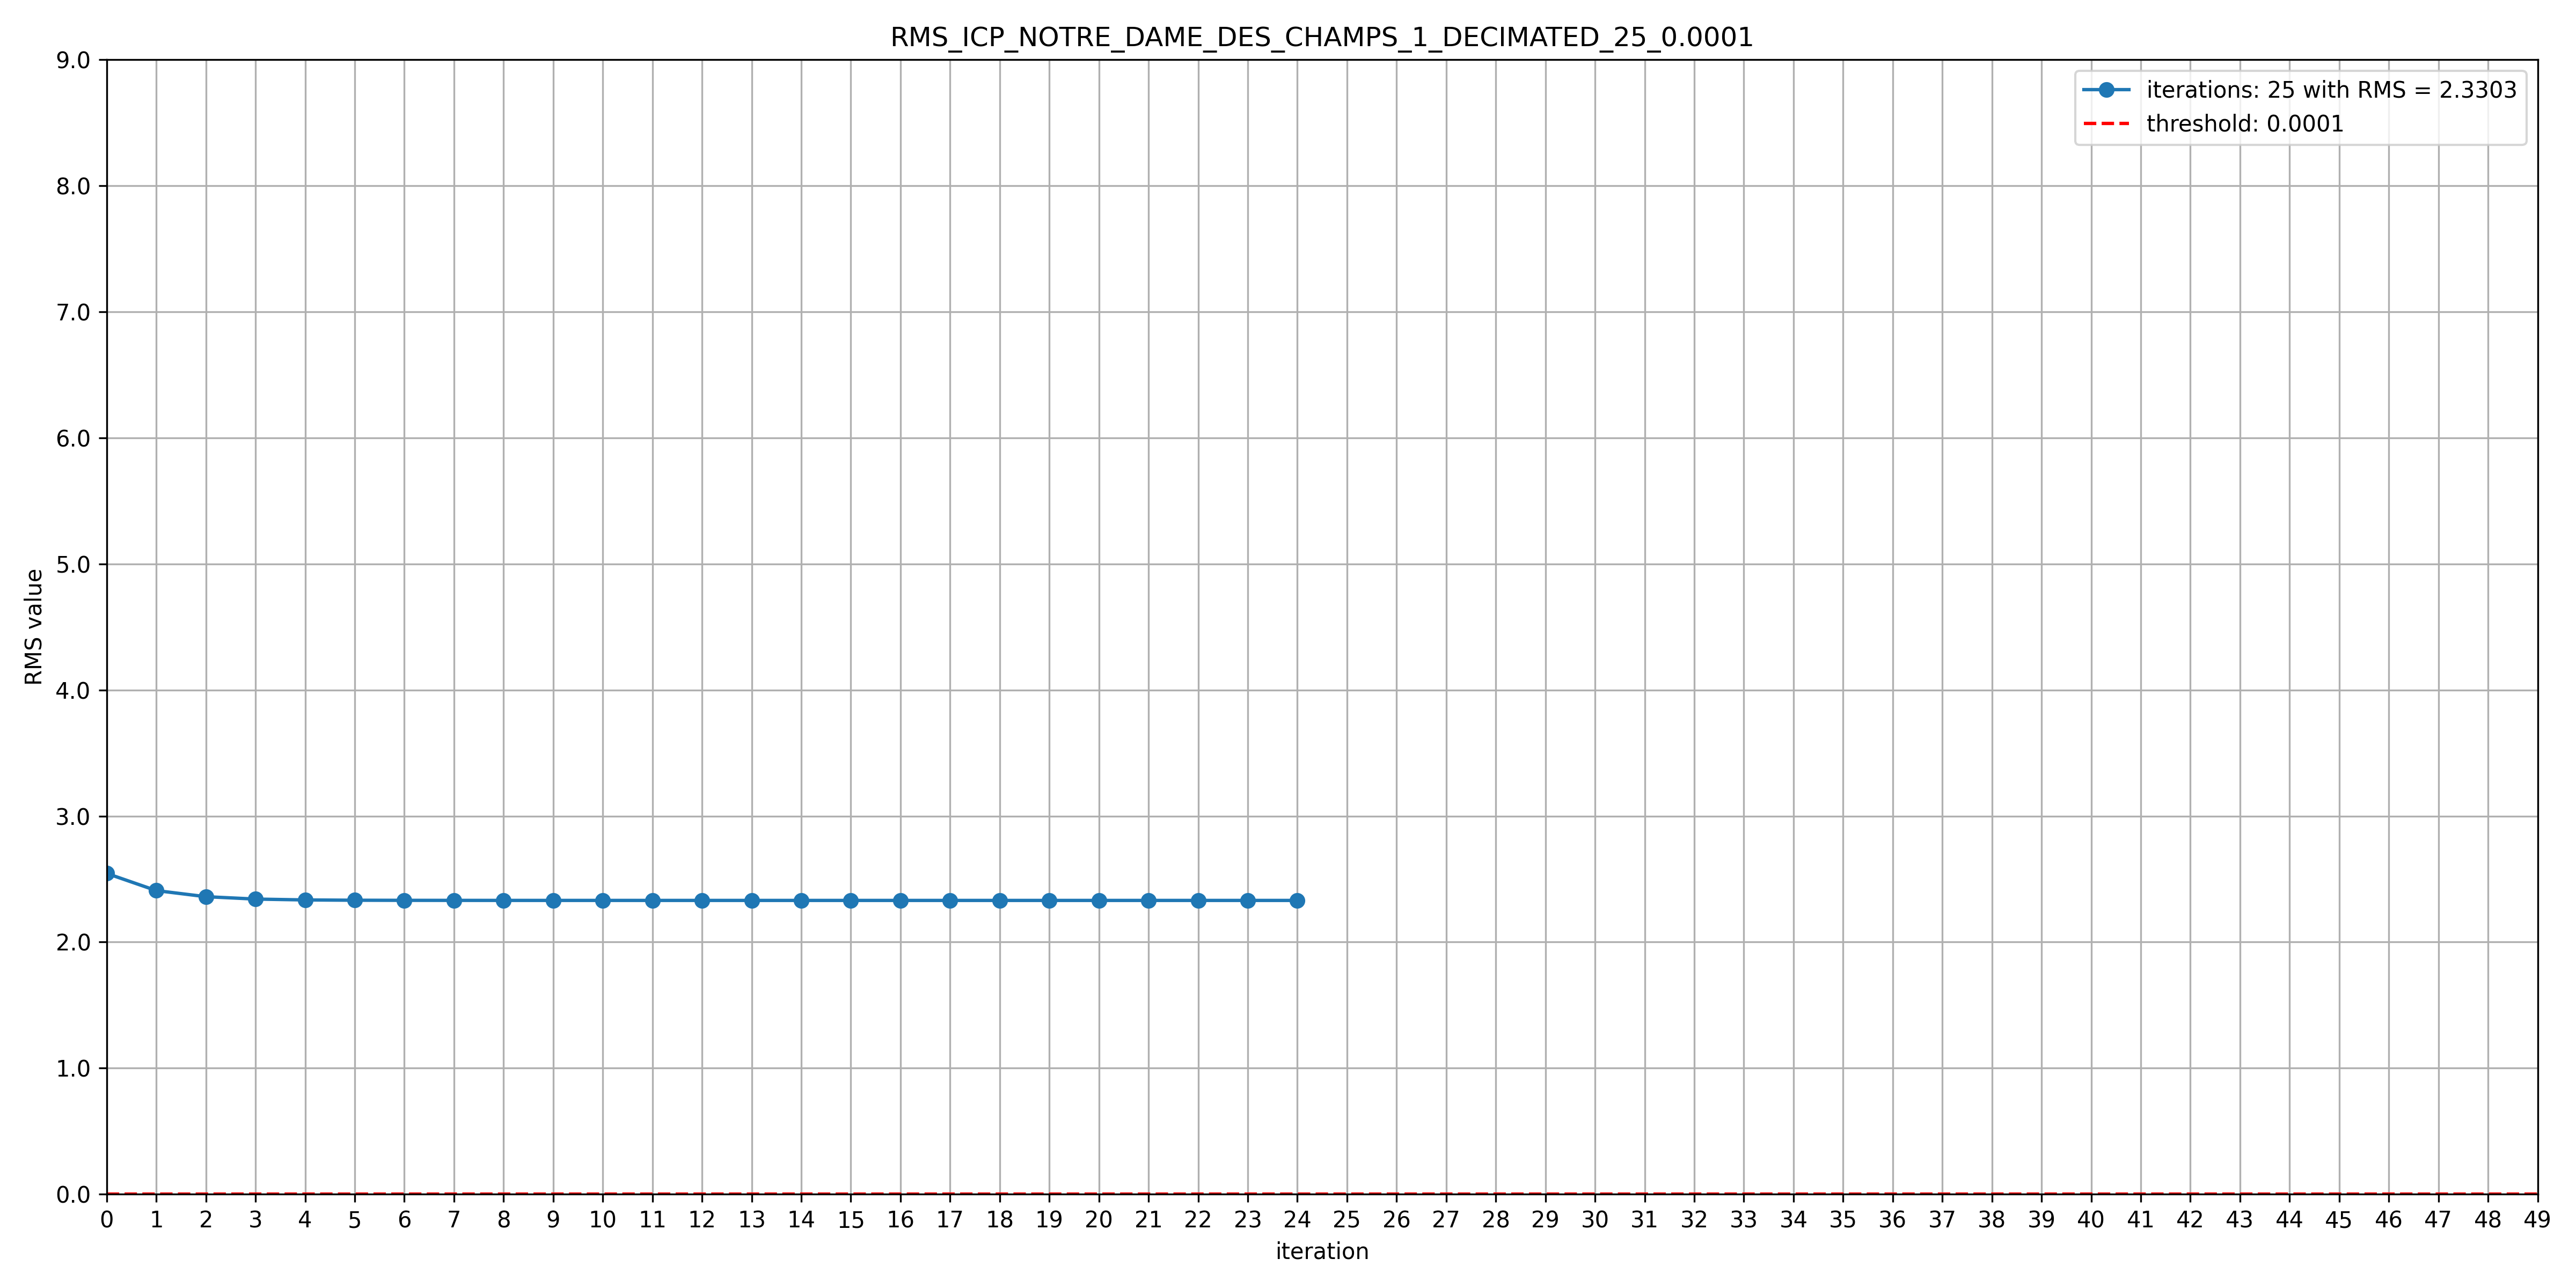
\includegraphics[width=\linewidth]{images/RMS_ICP_NOTRE_DAME_DES_CHAMPS_1_DECIMATED_25_0.0001.png}
        \caption{\texttt{NDC} decimated avec 25 iteractions}
        \label{}
    \end{subfigure}\hfill
    \begin{subfigure}[b]{0.475\textwidth}
        \centering
        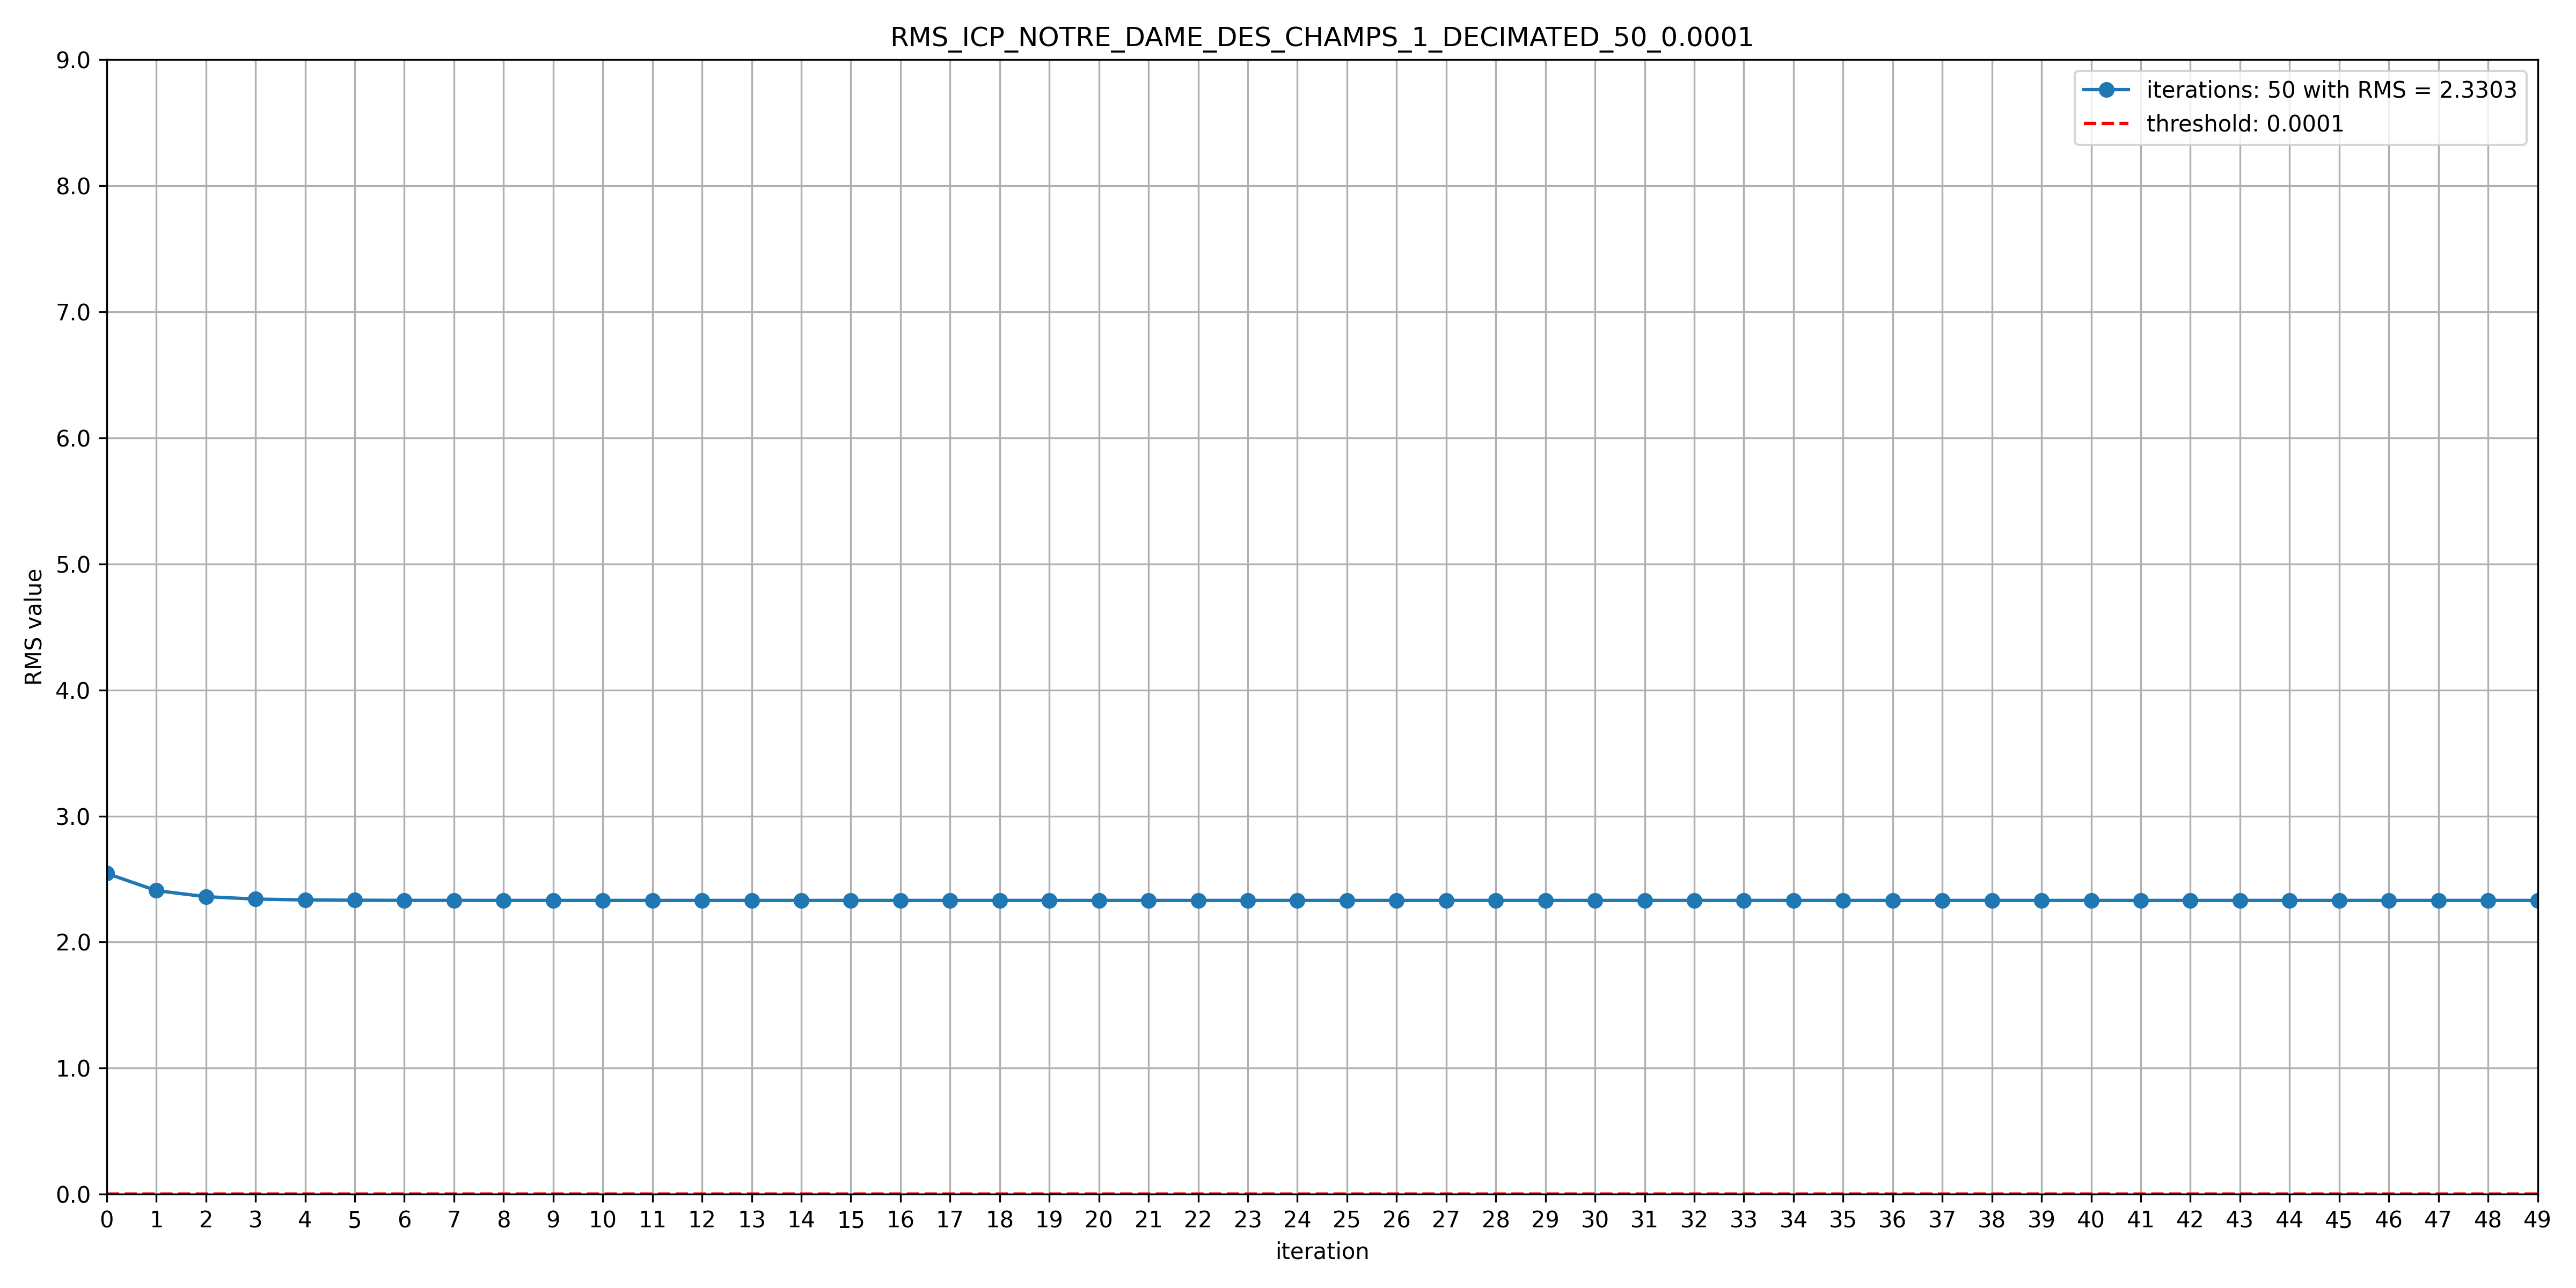
\includegraphics[width=\linewidth]{images/RMS_ICP_NOTRE_DAME_DES_CHAMPS_1_DECIMATED_50_0.0001.png}
        \caption{\texttt{NDC} decimated avec 50 iteractions}
        \label{}
    \end{subfigure}
    \caption{RMS pour différents executions de \texttt{compute\_ICP()}}
    \label{}
\end{figure}
\noindent Il est à noter que pour le nuage de points \texttt{Bunny} les résultats ont convergé rapidement, ne nécessitant que 19 itérations de l'algorithme ICP. Cependant, pour \texttt{Notre-Dame-des-Champs} non décimée, les résultats n'ont pas atteint le seuil et ont convergé vers une valeur élevée. On constate que, contrairement aux attentes, l’erreur RMS augmente avant de se stabiliser, ce qui indique que lorsqu’il y a de nombreux points, la méthode n’est pas recommandée en raison de son manque d’efficacité.

\begin{remark}
    Une erreur plus élevée pour \texttt{Notre-Dame-des-Champs} n'est pas surprenante puisque, étant donné les dimensions élevées du nuage de points, même de petites transformations peuvent générer de grandes variations entre 2 points, ce qui augmenterait généralement l'erreur.
\end{remark}

\noindent Le résultat pour \texttt{Notre-Dame-des-Champs} décimée a également été analysé, qui démontre également une erreur plus élevée et converge vers une valeur supérieure au seuil, mais dans ce cas l'erreur RMS présente un comportement attendu en diminuant à chaque interaction.

\begin{remark}
    Il convient de noter que l’utilisation de ICP est plus coûteuse en calcul et que l’utilisation de la version décimée était nécessaire pour réduire les temps de calcul.
\end{remark}

\noindent Cela démontre à quel point l'ICP nécessite des adaptations et une attention particulière car il ne sera pas toujours la meilleure alternative pour les nuages de points très denses comme dans le cas de \texttt{Notre-Dame-des-Champs}.
\end{document}
